\documentclass[a4paper, 12pt]{article}
\usepackage[portuguese]{babel}
\usepackage{chemist}
\usepackage{chemformula}
\usepackage{booktabs}
% Pacote para aceitar acentuação
\usepackage[utf8]{inputenc}
\usepackage{float}
% geometry, pacote para configurar as margens. 
% padrão ABNT => lmargin=3cm,tmargin=3cm,rmargin=2cm,bmargin=2cm
\usepackage[lmargin=3cm,tmargin=3cm,rmargin=2cm,bmargin=2cm]{geometry}
\setlength{\parindent}{0pt} % não identa a primeira linha

% graphicx = usar imagem (\includegraphics), comment = texto em formato de comentário, enumitem = enumeração, multirow e multicol = uso de tabelas, indentf = identar primeira linha
\usepackage{graphicx,xcolor,comment,enumitem,multirow,multicol,indentfirst}
\setlength{\parindent}{0pt} % não identa a primeira linha

% Pacotes para matemática
\usepackage{amsmath, amssymb, amsthm, amsfonts,  mathtools, amstext, nccmath}
\everymath{\displaystyle}

\usepackage[utf8]{inputenc}
\usepackage{hyperref}

%
% Título e autor do documento
%
\title{Química Analítica Quantitativa\\
	\large{\textbf{\\Volumetria de Neutralização \\
	Titulação de Ácido Acético com Hidróxido de Sódio}}
}

\author{Rogério Ribeiro Macêdo}
\date{\today}

\usepackage[font=scriptsize,labelfont=bf]{caption}
\usepackage{subcaption}
\usepackage{siunitx}

% draw a frame around given text
\newcommand{\framedtext}[1]{%
	\par%
	\noindent\fbox{%
		\parbox{\dimexpr\linewidth-2\fboxsep-2\fboxrule}{#1}%
	}%
}



\begin{document}
	\maketitle

\section{Objetivo}
O presente trabalho foi realizado objetivando aplicar a sequência de cálculos necessários à titulação do ácido acético (titulado) com hidróxido de sódio (titulante) e consequentemente gerar a curva de titulação. Lembrando que, para tal, por se tratar de um ácido fraco faz-se necessário a utilização da constante de dissociação do ácido (Ka). \\

A curva de titulação será construída relacionando o volume adicionado de NaOH com o valor do pH associado. 

\section{Etapas da titulação}
Antes de iniciar vale lembrar que o processo envolve basicamente 4 etapas e em cada uma delas o cálculo do pH é realizado considerando o contexto da titulação:

\begin{description}
	\item[\underline{Etapa 1}]: antes de iniciar a titulação \hfil \\ Neste ponto a solução contém apenas ácido acético. Portanto, o valor do pH é determinado pela dissociação do ácido.
	\item[\underline{Etapa 2}]: antes de atingir o ponto de equivalência \hfil \\ Ainda há ácido para reagir, assim, o pH é determinado pelo sistema tampão.
	\item[\underline{Etapa 3}]: no ponto de equivalência \hfil \\ O ponto de equivalência é o ponto onde todo o ácido reagiu com a base. O volume da base para isso é aquele que será determinado pelo volume de equivalência. O pH é determinado pela hidrólise do sal formado.
	\item[\underline{Etapa 4}]: depois do ponto de equivalência \hfil \\ Há excesso de base. O pH é determinado através desse excesso. A hidrólise do sal contribui pouco nesse ponto, pois o excesso de base reprime esta reação.
\end{description}

\section{Dados para titulação}

\begin{table}[H]
	\begin{center}
		\begin{tabular}{lp{5cm}lp{10cm}}\toprule
			& \textbf{Ácido Acético} & \textbf{Hidróxido de sódio} \\ \midrule			
			Volume & 50,00 mL & - \\ 
			Concentração & $0,100 \: mol \cdot L^{-1}$ & $0,100 \: mol \cdot L^{-1}$ \\ 
			Ka & $1,75 \times 10^{-5}$ & - \\
			\bottomrule
		\end{tabular}
	\end{center}
\end{table}

\section{Volume de equivalência}
O volume de equivalência é o volume necessário de titulante que irá reagir completamente com o titulado. No caso, o volume de NaOH necessário para reagir completamente com o ácido acético. O cálculo é realizado usando a expressão\footnote{C: concentração; V: volume}:

\begin{equation*}
	V_{titulante} \times C_{titulante} = V_{titulado} \times C_{titulado}
\end{equation*}

Portanto, o volume necessário de NaOH que será necessário para neutralizar todo o ácido acético será de:
\begin{fleqn}
\begin{align*}
	& V_{titulante} \times C_{titulante} = V_{titulado} \times C_{titulado} \\
	& V_{titulante} \times 0,100 = 50,00 \times 0,100 \\
	& V_{titulante} = 50,00 \text{ mL}
\end{align*}
\end{fleqn}

\section{Cálculos}
A partir deste ponto realizaremos os cálculos da titulação. Como o objetivo é construir a curva de titulação, os volumes que usaremos de NaOH serão pontuais. O conjunto de dados que será utilizado para a construção da curva pode ser encontrado no link: \href{https://github.com/rogerioribeiromacedo}{https://github.com/rogerioribeiromacedo/Chemistry}\footnote{https://github.com/rogerioribeiromacedo/Chemistry}

\subsection{No ponto inicial (sem adição de NaOH)}
O valor do Ka é considerado para a realização do cálculo, e este é calculado usando a expressão abaixo:
\begin{fleqn}
\begin{align*}
	Ka = \frac{[H_{3}O^{+}] \times [Ac^{-}]}{[HAc]}
\end{align*}
\end{fleqn}
Assim:
\begin{fleqn}
\begin{align*}
	& Ka = \frac{x \times x}{[HAc]} \\
	& Ka = \frac{x^{2}}{[HAc]} \\
	& x^{2} = Ka \times [HAc] \\
	& x = \sqrt{Ka \times [HAc]} \\
	& x = [H_{3}O^{+}] = \sqrt{(1,75 \times 10^{-5}) \times 0,100} \\
	& x = [H_{3}O^{+}] = 1,32 \times 10^{-3}
\end{align*}
\end{fleqn}
O valor do pH:
\begin{fleqn}
\begin{align*}
	& pH = - \log [H_{3}O^{+}] \\
	& pH = - \log {1,32 \times 10^{-3}} \\
	& \textbf{pH = 2,88}
\end{align*}
\end{fleqn}

\subsection{Antes do ponto de equivalência}
O cálculo do pH antes do ponto de equivalência faz uso da \textbf{Equação de Henderson-Hasselbalch}. Esta equação faz o relacionamento do pH de uma solução tampão, com o pKa, as concentrações da forma ácida (HAc) e da base conjugada ($Ac^{-}$). Abaixo a equação a ser utilizada:
\begin{fleqn}
\begin{align*}
	pH = pKa + \frac{[Ac^{-}]}{[HAc]}
\end{align*}
\end{fleqn}
Portanto, precisamos do pKa do ácido acético:
\begin{fleqn}
\begin{align*}
	& pKa = -log [Ka] \\
	& pKa = -log (1,75 \times 10^{-5}) \\
	& \textbf{pka = 4,757}
\end{align*}
\end{fleqn}

\subsection{Após adição de 0,05 mL (0,00005 L) de NaOH}
Esse volume representa o volume de uma única gota de NaOH adicionada na solução do titulante.

\begin{fleqn}
\begin{align*}
	& [Ac^{-}] = \frac{ V_{NaOH} \times C_{NaOH} }{ V_{HAc} + V_{NaOH} } = \frac{0,00005 \times 0,1}{0,05 + 0,00005} \\ \\
	& \mathbf{[Ac^{-}] = 0,0001 \text{ \textbf{mol}} \times L^{-1}}
\end{align*}
\end{fleqn}

\begin{fleqn}
\begin{align*}
	& [HAc] = \frac{ (C_{HAc} \times V_{HAc}) - (C_{NaOH} \times V_{NaOH}) }{ (V_{HAc} + V_{NaOH}) } = \frac{ (0,1 \times 0,05) - (0,1 \times 0,00005) }{ (0,05 + 0,00005) }\\ \\
	& \mathbf{[HAc] = 0,0998 \text{ \textbf{mol}} \times L^{-1}}
\end{align*}
\end{fleqn}

\begin{fleqn}
\begin{align*}
 	& pH = pKa + \log \frac{[Ac^{-}]}{[HAc]} = 4,757 + \log \frac{0,0001}{0,0998} \\
	& \textbf{pH = 1,758}
\end{align*}
\end{fleqn}

\subsection{Após adição de 0,1 mL (0,0001 L) de NaOH}
\begin{fleqn}
	\begin{align*}
		& [Ac^{-}] = \frac{ V_{NaOH} \times C_{NaOH} }{ V_{HAc} + V_{NaOH} } = \frac{0,0001 \times 0,1}{0,05 + 0,0001} \\ \\
		& \mathbf{[Ac^{-}] = 0,0001996 \text{ \textbf{mol}} \times L^{-1}}
	\end{align*}
\end{fleqn}

\begin{fleqn}
	\begin{align*}
		& [HAc] = \frac{ (C_{HAc} \times V_{HAc}) - (C_{NaOH} \times V_{NaOH}) }{ (V_{HAc} + V_{NaOH}) } = \frac{ (0,1 \times 0,05) - (0,1 \times 0,0001) }{ (0,05 + 0,0001) }\\ \\
		& \mathbf{[HAc] = 0,0996 \text{ \textbf{mol}} \times L^{-1}}
	\end{align*}
\end{fleqn}

\begin{fleqn}
	\begin{align*}
		& pH = pKa + \log \frac{[Ac^{-}]}{[HAc]} = 4,757 + \log \frac{0,0001996}{0,0996} \\
		& \textbf{pH = 2,0589}
	\end{align*}
\end{fleqn}

\subsection{Após adição de 10,00 mL (0,0001 L) de NaOH}
\begin{fleqn}
	\begin{align*}
		& [Ac^{-}] = \frac{ V_{NaOH} \times C_{NaOH} }{ V_{HAc} + V_{NaOH} } = \frac{0,1 \times 0,01}{0,05 + 0,01} \\ \\
		& \mathbf{[Ac^{-}] = 1,67 \times 10^{-2} \text{ \textbf{mol}} \times L^{-1}}
	\end{align*}
\end{fleqn}

\begin{fleqn}
	\begin{align*}
		& [HAc] = \frac{ (C_{HAc} \times V_{HAc}) - (C_{NaOH} \times V_{NaOH}) }{ (V_{HAc} + V_{NaOH}) } = \frac{ (0,1 \times 0,05) - (0,1 \times 0,01) }{ (0,05 + 0,01) }\\ \\
		& \mathbf{[HAc] = 6,67 \times 10^{-2} \text{ \textbf{mol}} \times L^{-1}}
	\end{align*}
\end{fleqn}

\begin{fleqn}
	\begin{align*}
		& pH = pKa + \log \frac{[Ac^{-}]}{[HAc]} = 4,757 + \log \frac{1,67 \times 10^{-2}}{6,67 \times 10^{-2}} \\
		& \textbf{pH = 4,156}
	\end{align*}
\end{fleqn}

\subsection{Após adição de 25,00 mL (0,025 L) de NaOH}
Esse volume corresponde à metade do volume de equivalência, portanto, nesse ponto, o valor do pH corresponde ao valor do pKa. Assim:

\begin{fleqn}
	\begin{align*}
		 \textbf{pH = pKa = 4,757}
	\end{align*}
\end{fleqn}

\section{Curva de titulação}
A curva de titulação é resultado de programa escrito em Python, que, utilizando os passos descritos na seção \textbf{Etapas de titulação}, produziu os dados necessários para sua construção. \\

O programa toma como referência os dados para titulação da seção 3 e calcula o pH considerando a variação de volume do NaOH de 0,00 mL até 120 mL. Abaixo, podemos ver os primeiros e últimos valores deste cálculo:

\begin{table}[H]
	\begin{center}
		\begin{tabular}{lp{5cm}lp{10cm}}\toprule
			& \textbf{pH} & \textbf{Volume (L)} \\ \midrule			
			& 2.87848000000 & 0.00000000000 \\ 
			& 1.75740000000	& 0.00005000000 \\ 
			& 2.05886000000	& 0.00010000000 \\
			& 2.23539000000	& 0.00015000000 \\
			& 2.36076000000	& 0.00020000000 \\
			& ... & ... \\
			& 12.61556000000 & 0.12025000000 \\
			& 12.61574000000 & 0.12030000000 \\
			& 12.61592000000 & 0.12035000000 \\
			& 12.61610000000 & 0.12040000000 \\
			& 12.61628000000 & 0.12045000000 \\			
			\bottomrule
		\end{tabular}
	\end{center}
\end{table}



%
%
%\begin{table}[H]
%	\begin{center}
%		\begin{tabular}{lp{5cm}lp{10cm}}\toprule
%			& pH & Volume & \\ 
%			\midrule			
%			& 2.87848000000	& 0.00000000000 & \\
%			& 1.75740000000	& 0.00005000000 & \\ 
%			& 2.05886000000	& 0.00010000000 & \\
%			& 2.23539000000	& 0.00015000000 & \\
%			& 2.36076000000	& 0.00020000000 & \\
%			& ... & ... & \\
%			& 12.61556000000	& 0.12025000000 & \\
%			& 12.61574000000	& 0.12030000000 & \\
%			& 12.61592000000	& 0.12035000000 & \\
%			& 12.61610000000	& 0.12040000000 & \\
%			& 12.61628000000	& 0.12045000000 & \\
%			\bottomrule
%		\end{tabular}
%	\end{center}
%\end{table}

\section{Gráfico}

\begin{figure}[H]
	\centering
	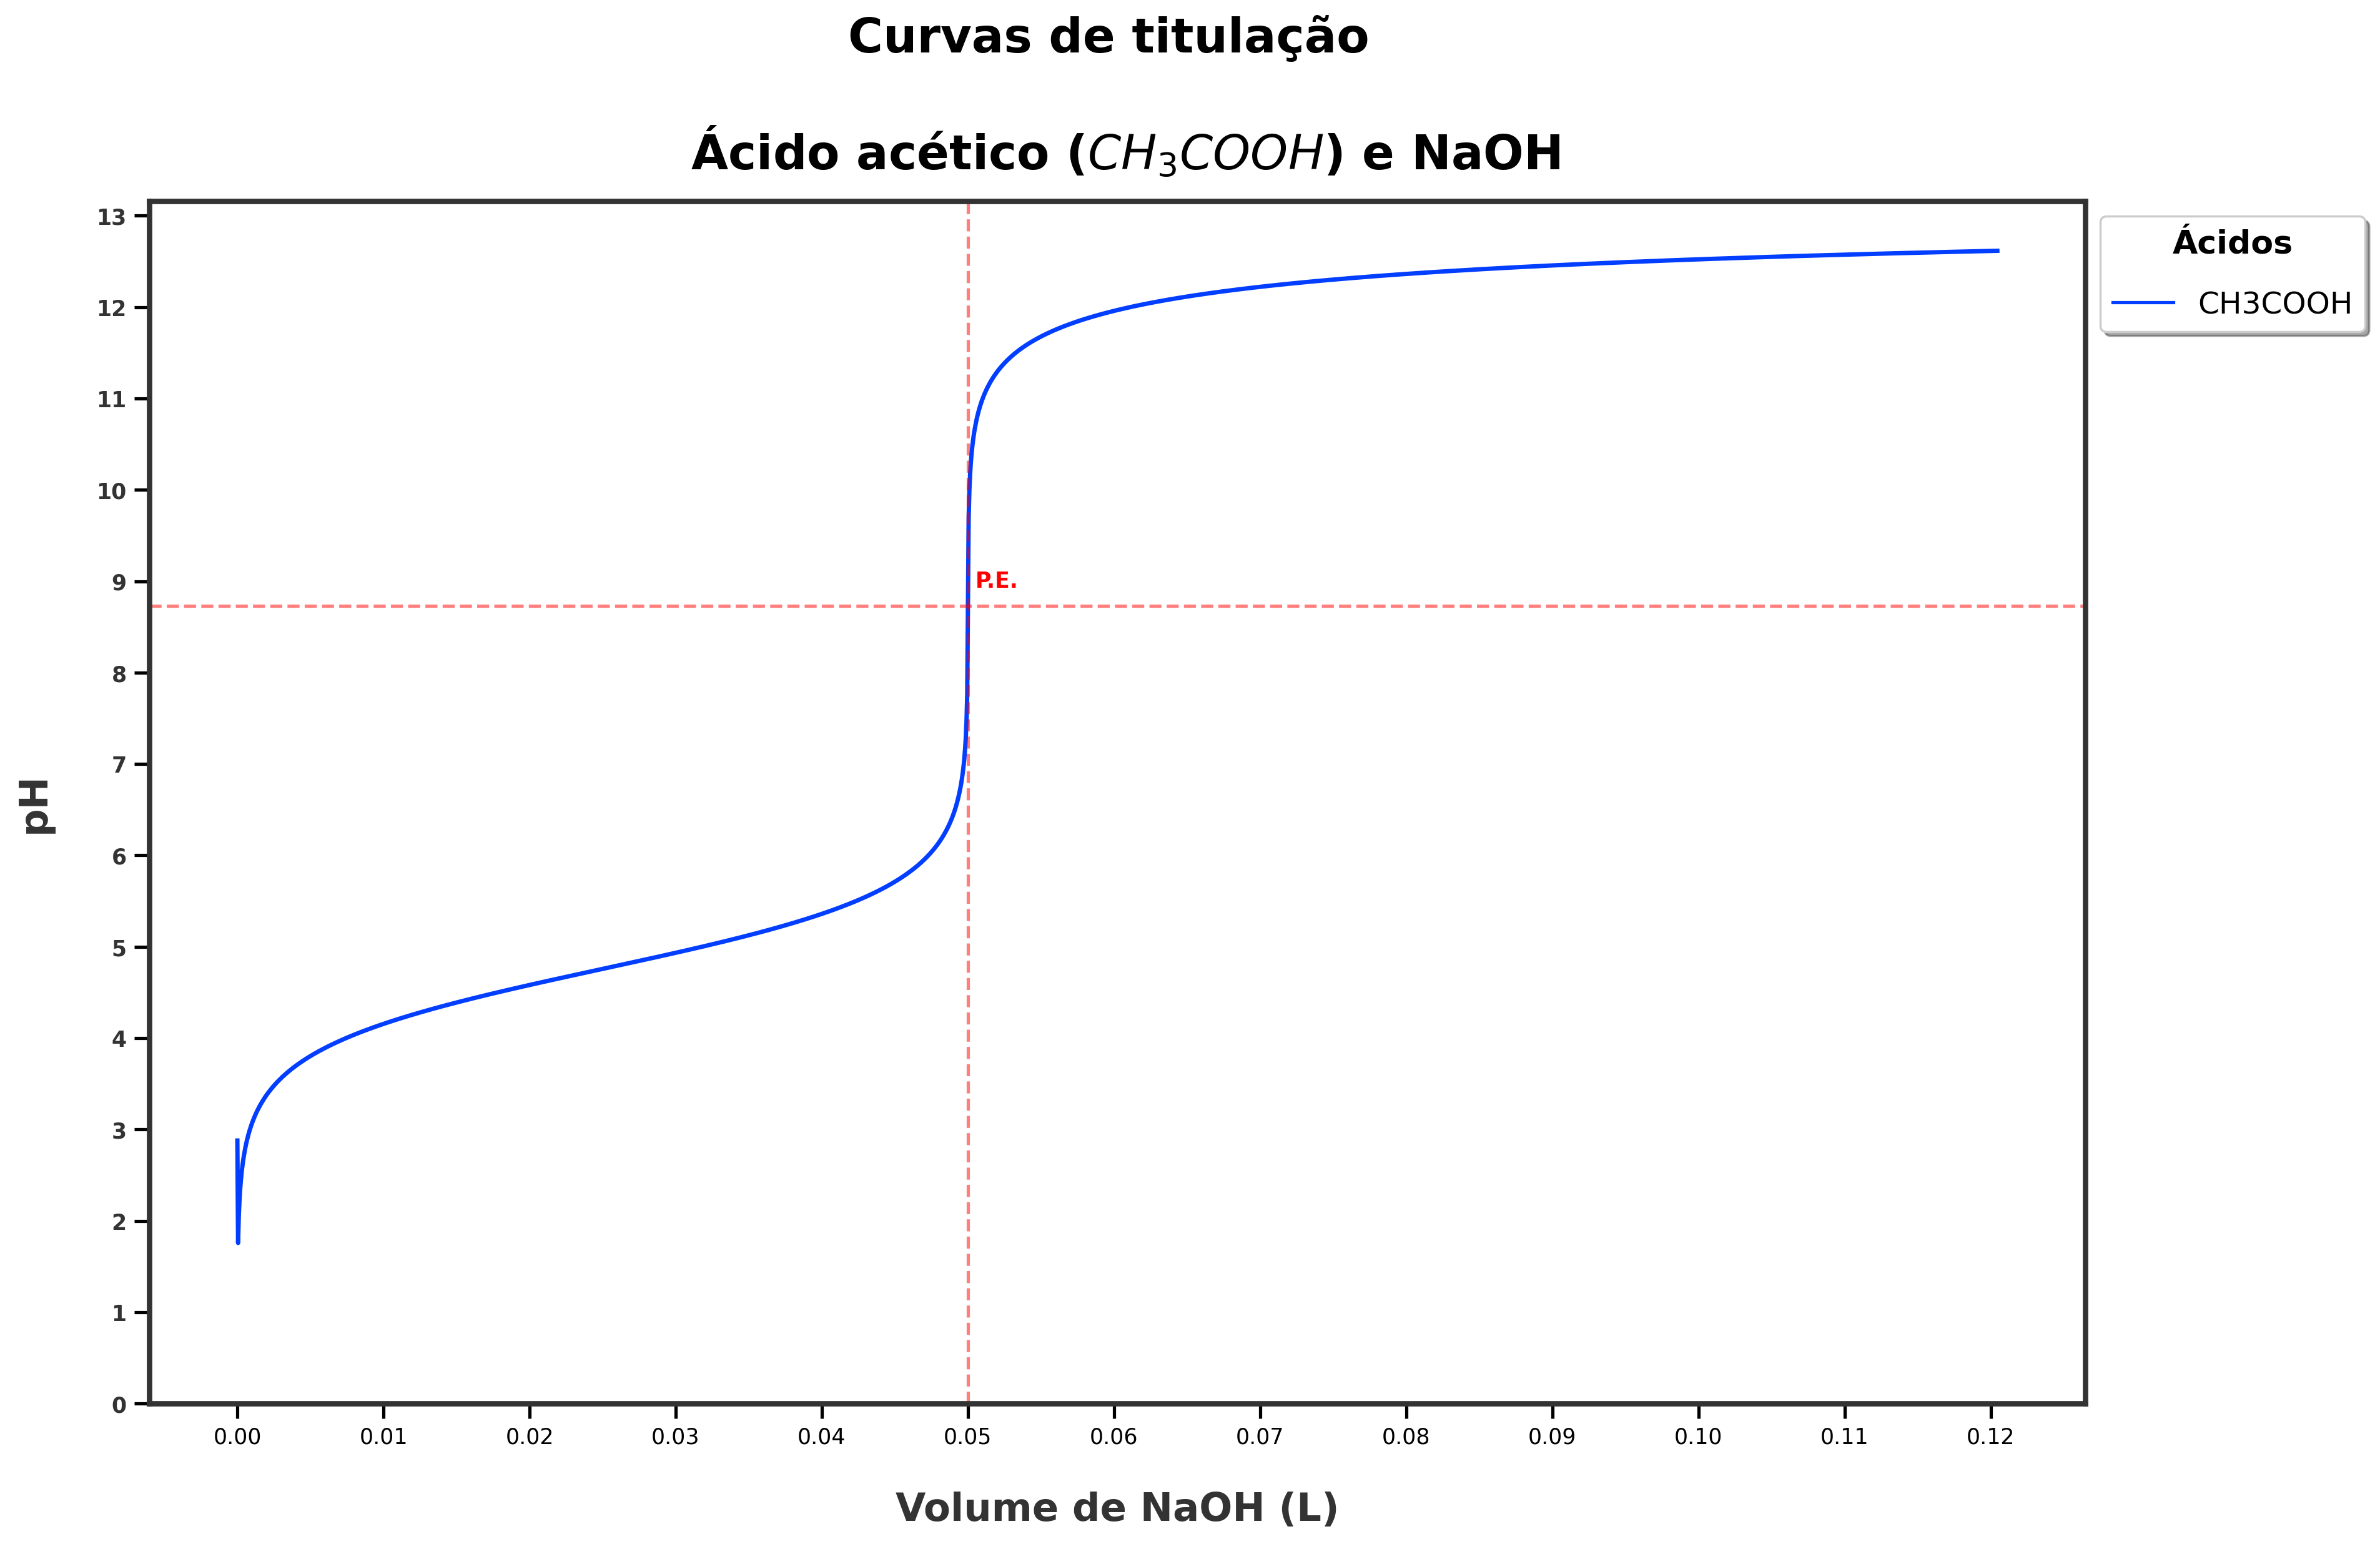
\includegraphics[width=0.99\linewidth]{../curva_de_titulacao_ac_acetico}
	\caption[Curva de titulação]{}
	\label{fig:curvadetitulacaoacacetico}
\end{figure}



\end{document}